\documentclass[10pt]{article}

\usepackage{hyperref}
\usepackage{enumerate}
\usepackage{amsmath}
\usepackage{graphicx}
% --------------------------------------------------------------
\title{A very simple latex doccument \\
\textbf{Quadratic equation}}
\author{Tiep Vu}
\date{July 2016}

\begin{document}
\maketitle

\section{Problem} % (fold)
\label{sec:problem}
	Given three real numbers $a, b, c$, solve the equation: 
	\begin{equation}
	\label{eqn: problem}
	    ax^2 + bx + c = 0.
	\end{equation}
% section problem (end)

\section{Solution} % (fold)
\label{sec:solution}
We consider two cases: 
\begin{enumerate}
	\item $a = 0$.
	\begin{itemize}
		\item If $ b = 0, c = 0 \Rightarrow$ solution is $x \in R$ 

		\item If $ b = 0, c \neq 0 \Rightarrow$ there no $x$ satisfying equation 
		(\ref{eqn: problem}). 

		\item If $\displaystyle b \neq 0 \Rightarrow x = -\frac{c}{b}$
	\end{itemize}
	\item $a \neq 0$. Let $\Delta = b^2 - 4ac.$
	\begin{equation}
	\label{eqn:solution}
		\displaystyle
	    x = \left\{
	    	% \begin{matrix}
	    	\begin{array} {cl}
	    		
	    		\displaystyle \frac{-b \pm \sqrt{\Delta}}{2a} & \text{if~} \Delta > 0. \\
	    		\displaystyle \frac{-b}{2a}                   & \text{if~} \Delta = 0 \\
	    		\displaystyle 0                               & \text{other wise}
	    	\end{array}
	    	% \end{matrix}
		    \right. 	
	\end{equation}
\end{enumerate}
% section solution (end)

\section{Example} % (fold)
\label{sec:example}
Find $x-$intercepts of the graph $y = x^2 - x - 2$.
\\
\begin{enumerate}
	\item Using graph shown in Figure \ref{fig:graph1}. \\
	\begin{figure}[!h]  		 
	\label{fig:graph1}
	\centering
	 	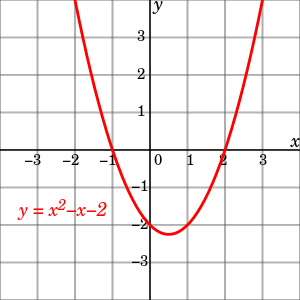
\includegraphics[scale = .3]{figs/fig1.png} 
	 	\caption{Caption is here}
	\end{figure}
	The solution is $x \in \{1, 2\}$
	\item Using (\ref{eqn:solution}). 
	We need to solve the following quadratic equation: 
	\begin{equation}
	    x^2 - x - 2 = 0.
	\end{equation}
	$\Rightarrow$ solution $x \in \{-1, 2\}$.
\end{enumerate}

\section{More examples} % (fold)
\label{sec:more_examples}
Given $a, b, c$, find $x$:

\begin{table}[!h]
\centering
\caption{My caption}
\label{my-label}
\begin{tabular}{|l|l|l||l|l|}
\hline
$a$ & $b$  & $c$ & $x_1$ & $x_2$ \\ \hline \hline 
1 & -4 & 3 & 1    & 3    \\ \hline
1 & -2 & 1 & 1    & 1    \\ \hline
\end{tabular}
\end{table}

\section{Citations} % (fold)
\label{sec:citations}

% section citations (end)
\cite{vu2015dfdl}


% section more_examples (end)

% section example (end)

\bibliographystyle{IEEEtran}
\bibliography{refs}
\end{document}